\chapter{Methodology}\label{chap:Methodology}

\section*{Problem Formulation}

\begin{figure}[H]
    \centering
    \begin{tikzpicture}[
        auto,
        block/.style={rectangle, draw, fill=blue!20, text width=6em, text centered, rounded corners, minimum height=4em},
        line/.style={draw, -latex'}
    ]
        % Nodes
        \node[block, text width=8em] (inputs) {Inputs\\- Grid Map\\- Robot States\\- Parameters};
        \node[block, right=2cm of inputs] (planner) {Path Planner (Optimizer)};
        \node[block, above=1cm of planner, text width=10em] (objective) {Objective Function\\- Coverage\\- Connectivity\\- Penalties};
        \node[block, below=1cm of planner, text width=8em] (constraints) {Constraints\\- Map Bounds\\- Motion\\- Energy\\- Obstacles\\- Collisions};
        \node[block, right=2cm of planner] (outputs) {Optimal Trajectories};

        % Arrows
        \path [line] (inputs) -- (planner);
        \path [line] (objective) -- (planner);
        \path [line] (constraints) -- (planner);
        \path [line] (planner) -- (outputs);
    \end{tikzpicture}
    \caption{High-level overview of the path planning optimization approach.}
    \label{fig:optimization_overview}
\end{figure}

This chapter presents the mathematical formulation of the multi-robot exploration problem with distance-weighted connectivity constraints and energy limitations. We model the environment as a discrete grid and formulate the problem as a constrained optimization that balances area coverage with maintaining communication links between robots, while accounting for battery constraints and penalizing undesirable behaviors such as network disconnection and obstacle encounters.

\subsection*{Assumptions}

The environment is represented as a grid map $M \in \{0,1,2,3\}^{n \times m}$ with unit cells of size $1\times 1$. Each cell $M[x,y]$ takes values: $M[x,y]=0$ means unexplored, $M[x,y]=1$ means free space, $M[x,y]=2$ means obstacle, and $M[x,y]=3$ marks a cell occupied by a robot.

We assume that all robots are exactly identical in their capabilities, including sensing range, communication radius, motion constraints, and battery capacity. This makes coordination simpler and ensures fairness in task allocation, as no robot has advantages over others.

We assume that obstacles are unknown at the start, which matches realistic exploration scenarios where the environment structure is discovered gradually. As robots explore, newly detected obstacles are shared among all robots through their communication network. Let $O_t \subseteq \{(x,y) \mid 1 \le x \le n, 1 \le y \le m\}$ denote the set of known obstacle locations at time $t$, with $O_t \subseteq O_{t+1}$ for all $t \ge 0$. This monotonic growth of obstacle knowledge captures the fact that once an obstacle is discovered, it remains known. When a robot encounters an obstacle during execution, it uses a reactive obstacle avoidance strategy to navigate around the obstruction while trying to maintain its overall trajectory toward the planned goal.

Robots are modeled as point agents that move synchronously at discrete time steps $t \in \{0,1,2,\ldots\}$. Motion follows a 4-connected grid topology (up, down, left, right) or allows robots to stay in place. This discretization simplifies planning while maintaining sufficient capability for typical robotic platforms.

Each robot is equipped with a battery that permits movement for a maximum of $\ell \in \mathbb{N}$ cells, where $\ell > 0$ represents the energy budget. Since all robots are identical, they share the same energy capacity. This constraint reflects the practical limitation that robots must complete their exploration mission within their available energy resources.

We assume robots share their positions at each time step through local communication. The desirability of maintaining communication between any pair of robots is modeled by a weight function that decreases with their Euclidean distance, reflecting the fact that closer robots have more reliable communication links.

\subsection*{Map, Robots, and Positions}

There are $N \in \mathbb{N}$ robots indexed by $i \in \{1,\ldots,N\}$. The position of robot $i$ at time $t$ is denoted
\[
    p_{i,t} = (x_{i,t}, y_{i,t}) \in \mathbb{Z}^2,
\]
where
\[
    x_{i,t} \in \{1,\ldots,n\}, \qquad y_{i,t} \in \{1,\ldots,m\}.
\]
Initial positions $p_{i,0}$ are given for all $i \in \{1,\ldots,N\}$.

The discrete grid representation allows us to formulate the problem as a mixed-integer program. Each robot's state at any time is fully described by its integer coordinates within the map boundaries.

The 4-connected motion constraint is enforced by the Manhattan distance:
\[
    |x_{i,t}-x_{i,t-1}| + |y_{i,t}-y_{i,t-1}| \le 1, \qquad \forall i \in \{1,\ldots,N\},\; \forall t \ge 1.
\]

This constraint ensures that each robot can move at most one grid cell per time step in one of the four cardinal directions, or remain stationary. The Manhattan distance metric naturally captures the 4-connected neighborhood structure and prevents diagonal movements, which simplifies motion planning and collision avoidance.

\subsection*{Energy Consumption Model}

To model battery constraints, we define the cumulative distance traveled by robot $i$ up to time $t$ as:
\[
    D_{i,t} = \sum_{\tau=1}^{t} \left(|x_{i,\tau}-x_{i,\tau-1}| + |y_{i,\tau}-y_{i,\tau-1}|\right), \qquad \forall i \in \{1,\ldots,N\},\; \forall t \ge 1.
\]

Each unit of movement (one grid cell) consumes one unit of battery. The energy constraint for each robot is:
\[
    D_{i,t} \le \ell, \qquad \forall i \in \{1,\ldots,N\},\; \forall t \ge 0,
\]
where $\ell \in \mathbb{N}$ is the maximum number of cells each robot can traverse.

This formulation ensures that the total distance traveled by any robot never exceeds its battery capacity. The constraint applies at every time step, meaning that robots must stop moving once they have exhausted their energy budget. Since robots are identical, they all share the same energy limit $\ell$. This constraint forces the planner to balance exploration goals with energy availability, potentially requiring some robots to remain stationary or return to already-explored areas to conserve energy for critical coordination tasks. The mission effectively ends when all robots have either exhausted their batteries or completed the exploration task.

\subsection*{Coverage and Distance-Weighted Connectivity}

Coverage is a fundamental metric in exploration tasks, measuring the fraction of the environment that has been visited by at least one robot. We define the binary coverage variable $C_{x,y} \in \{0,1\}$ for each cell $(x,y)$:
\[
C_{x,y} =
\begin{cases}
1, & \text{if } \exists\, i \in \{1,\ldots,N\},\, \exists\, t \ge 0 \text{ such that } p_{i,t} = (x,y), \\
0, & \text{otherwise.}
\end{cases}
\]

The coverage is enforced via indicator constraints:
\[
C_{x,y} \;\ge\; \mathbb{I}\!\left[p_{i,t} = (x,y)\right], \quad \forall x \in \{1,\ldots,n\},\; \forall y \in \{1,\ldots,m\},\; \forall i \in \{1,\ldots,N\},\; \forall t \ge 0,
\]
where $\mathbb{I}[\cdot]$ is the indicator function that equals 1 when its argument is true and 0 otherwise.

These constraints ensure that once a cell is visited by any robot at any time, its coverage variable is set to 1 and remains 1 thereafter. This formulation naturally handles the cumulative nature of coverage: a cell needs to be visited only once to be considered covered, regardless of whether robots later leave or return to it.

To model communication quality between robots, we first define the Euclidean distance between robots $i$ and $j$ at time $t$ as:
\[
d_{ij,t} \;=\; \sqrt{(x_{i,t}-x_{j,t})^2 + (y_{i,t}-y_{j,t})^2} \in \mathbb{R}_{\ge 0}.
\]

Building on this, we define the distance-weighted link quality $W_{ij,t} \in [0,1]$ as:
\[
W_{ij,t} \;=\; 
\begin{cases}
\dfrac{1}{1+d_{ij,t}}, & \text{if } d_{ij,t} \le R_c, \\[6pt]
0, & \text{if } d_{ij,t} > R_c,
\end{cases}
\]
where $R_c > 0$ is the communication radius threshold.

This formulation captures two important aspects of real-world communication: (1) link quality degrades continuously with distance within communication range, following an inverse relationship, and (2) beyond a critical distance $R_c$, communication becomes impossible. The weight $W_{ij,t}$ reaches its maximum value of 1 when robots are at the same location ($d_{ij,t}=0$) and decreases smoothly as distance increases, encouraging the optimizer to keep robots reasonably close while exploring.

\subsection*{Network Connectivity and Disconnection Penalty}

Define the edge set at time $t$ as:
\[
    E_t = \left\{(i,j) \;\big|\; i,j \in \{1,\ldots,N\},\; i < j,\; d_{ij,t} \leq d_{\text{threshold}}\right\}, \quad \forall t \ge 0,
\]
where $d_{\text{threshold}} > 0$ is the connectivity distance threshold.

Let $G_t = (V, E_t)$ be the communication graph at time $t$, where $V = \{1,\ldots,N\}$ is the set of robot indices. We define $\mathcal{C}_t$ as the set of connected components in $G_t$. For each robot $i$, let $C_t(i)$ denote the connected component containing robot $i$ at time $t$.

To measure network disconnection, we introduce a binary indicator variable:
\[
    \delta_{i,t} = 
    \begin{cases}
    1, & \text{if robot } i \text{ is disconnected from the main network at time } t, \\
    0, & \text{otherwise,}
    \end{cases}
\]
where the "main network" is defined as the largest connected component in $G_t$ (breaking ties arbitrarily). Formally:
\[
    \delta_{i,t} = \mathbb{I}\!\left[C_t(i) \neq \arg\max_{C \in \mathcal{C}_t} |C|\right], \qquad \forall i \in \{1,\ldots,N\},\; \forall t \ge 0.
\]

When a robot is disconnected, we measure its distance to the main network. Let $V_{\text{main},t} \subseteq V$ denote the set of robots in the main network at time $t$. The distance from disconnected robot $i$ to the main network is:
\[
    d_{i,\text{net},t} = \min_{j \in V_{\text{main},t}} d_{ij,t}, \qquad \forall i \in \{1,\ldots,N\} \text{ with } \delta_{i,t}=1.
\]

Since the mission continues until all robots exhaust their energy or complete exploration, we compute the total disconnection penalty by summing over all robots and all time steps up to the maximum mission duration $T_{\text{max}}$:
\[
    P_{\text{disconnect}} = \sum_{t=0}^{T_{\text{max}}} \sum_{i=1}^{N} \delta_{i,t} \cdot d_{i,\text{net},t},
\]
where $T_{\text{max}} = \max\{\ell, nm\}$ is an upper bound on mission duration (either all energy is depleted or all cells are explored).

This penalty term has two important properties: (1) it is zero when all robots remain connected throughout the mission, and (2) when disconnection occurs, the penalty scales linearly with how far the isolated robot(s) are from the main network. This encourages the planner to either maintain full connectivity or, if temporary disconnection is unavoidable, to minimize both the duration and severity (distance) of the disconnection. Robots that are only slightly beyond communication range incur smaller penalties than those that have wandered far from the team.

\subsection*{Obstacle Encounter Penalty}

To discourage robots from planning paths that lead to obstacle encounters, we define an obstacle encounter indicator:
\[
    \eta_{i,t} = 
    \begin{cases}
    1, & \text{if robot } i \text{ encounters an obstacle at time } t, \\
    0, & \text{otherwise.}
    \end{cases}
\]

An obstacle encounter occurs when a robot plans to move to a cell that is later discovered to contain an obstacle. Formally, robot $i$ encounters an obstacle at time $t$ if:
\[
    p_{i,t} \in O_t \setminus O_{t-1}, \qquad \text{for } t \ge 1.
\]

This captures newly discovered obstacles that were unknown during planning. When such an encounter occurs, the robot must reactively navigate around the obstacle, leading to suboptimal paths, wasted energy, and delays.

The total obstacle encounter penalty is:
\[
    P_{\text{obstacle}} = \sum_{t=1}^{T_{\text{max}}} \sum_{i=1}^{N} \eta_{i,t}.
\]

This penalty counts the total number of obstacle encounters across all robots and all time steps. While it is impossible to completely avoid obstacles that are initially unknown, this penalty term encourages the planner to favor paths through regions with lower perceived obstacle density (based on prior exploration) and to coordinate robot movements such that scouts discover obstacles ahead of the main group. The penalty also indirectly encourages more conservative exploration strategies that reduce the likelihood of unexpected collisions.

\subsection*{Objective Function}

The optimization problem seeks to maximize a composite objective that balances exploration, connectivity, energy efficiency, and safety:
\[
    \max\; f \;=\;
    \underbrace{\alpha \sum_{x=1}^{n}\sum_{y=1}^{m} C_{x,y}}_{\text{coverage term}}
    \;+\;
    \underbrace{\beta \sum_{t=0}^{T_{\text{max}}}\sum_{i=1}^{N-1}\sum_{j=i+1}^{N} W_{ij,t}}_{\text{distance-weighted connectivity term}}
    \;-\;
    \underbrace{\gamma \cdot P_{\text{disconnect}}}_{\text{disconnection penalty}}
    \;-\;
    \underbrace{\zeta \cdot P_{\text{obstacle}}}_{\text{obstacle encounter penalty}},
\]
where $\alpha, \beta, \gamma, \zeta \in \mathbb{R}_{>0}$ are positive weighting parameters.

The first term rewards exploring new areas by counting the total number of covered cells. The second term encourages robots to maintain proximity throughout the mission by accumulating link quality weights over all time steps and all robot pairs. The third term penalizes network fragmentation, with penalties scaled by the distance of disconnected robots from the main network. The fourth term discourages obstacle encounters, which lead to inefficient reactive behaviors.

The parameters $\alpha, \beta, \gamma, \zeta$ allow us to tune the relative importance of these competing objectives. Larger $\alpha$ prioritizes aggressive exploration potentially at the cost of team fragmentation and safety. Larger $\beta$ keeps the team cohesive but may slow down exploration. Larger $\gamma$ enforces stricter connectivity requirements, particularly penalizing scenarios where robots become isolated far from the team. Larger $\zeta$ promotes more cautious exploration strategies that reduce collision risk. The choice of these parameters depends on mission requirements: search-and-rescue operations might prioritize coverage ($\alpha$) and connectivity ($\beta$, $\gamma$), while mapping missions in hazardous environments might additionally emphasize safety ($\zeta$).

\subsection*{Constraints}

The optimization is subject to several constraints that ensure feasible and safe robot trajectories.

\begin{enumerate}
    \item \textbf{Map bounds:}
    \[
        x_{i,t} \in \{1,\ldots,n\}, \qquad y_{i,t} \in \{1,\ldots,m\}, \qquad \forall i \in \{1,\ldots,N\},\; \forall t \ge 0.
    \]
    
    These constraints ensure that all robots remain within the boundaries of the defined map at all times. Violating these bounds would place robots in undefined regions outside the environment.
    
    \item \textbf{Motion constraint (4-connectivity):}
    \[
        |x_{i,t}-x_{i,t-1}| + |y_{i,t}-y_{i,t-1}| \le 1, \qquad \forall i \in \{1,\ldots,N\},\; \forall t \ge 1.
    \]
    
    This constraint enforces the kinematic limits of the robots, ensuring that position changes between consecutive time steps are physically realizable. The Manhattan distance bound of 1 permits movement to any of the four adjacent cells or staying in place, but prohibits diagonal moves and larger jumps.
    
    \item \textbf{Energy budget:}
    \[
        D_{i,t} = \sum_{\tau=1}^{t} \left(|x_{i,\tau}-x_{i,\tau-1}| + |y_{i,\tau}-y_{i,\tau-1}|\right) \le \ell, \qquad \forall i \in \{1,\ldots,N\},\; \forall t \ge 0.
    \]
    
    This constraint ensures that the total distance traveled by each robot at any time does not exceed its battery capacity $\ell$. Since all robots are identical, they share the same energy limit. This forces the planner to make strategic decisions about which regions to explore and which robots should undertake longer journeys versus remaining in supporting roles. Once a robot reaches its energy limit, it must remain stationary for the remainder of the mission.
    
    \item \textbf{Obstacle avoidance (with online discovery):}
    \[
        p_{i,t} \notin O_t, \qquad \forall i \in \{1,\ldots,N\},\; \forall t \ge 0,
    \]
    where $O_t \subseteq O_{t+1}$ for all $t \ge 0$.
    
    These constraints prevent robots from planning to occupy cells containing known obstacles. Since obstacles are discovered gradually ($O_t \subseteq O_{t+1}$), the constraint set grows over time as exploration proceeds. This formulation naturally handles the online nature of the problem: robots must avoid all obstacles known at time $t$ when planning their position at time $t$, but cannot anticipate obstacles that will only be discovered later. When a robot encounters a previously unknown obstacle during execution (triggering the obstacle encounter penalty $P_{\text{obstacle}}$), it uses reactive obstacle avoidance to navigate around the obstruction.
    
    \item \textbf{Collision avoidance:}
    \[
        p_{i,t} \neq p_{j,t}, \qquad \forall i,j \in \{1,\ldots,N\} \text{ with } i \neq j,\; \forall t \ge 0.
    \]
    
    This constraint ensures that no two robots occupy the same cell simultaneously, preventing inter-robot collisions. Combined with the motion constraints, this also implicitly prevents certain types of edge collisions where robots would swap positions in a single time step.
    
    \item \textbf{Coverage update:}
    \[
        C_{x,y} \;\ge\; \mathbb{I}\!\left[p_{i,t} = (x,y)\right], \quad \forall x \in \{1,\ldots,n\},\; \forall y \in \{1,\ldots,m\},\; \forall i \in \{1,\ldots,N\},\; \forall t \ge 0.
    \]
    
    These constraints link the coverage variables to the robot positions, ensuring that the coverage term in the objective function accurately reflects the set of visited cells. Since $C_{x,y}$ appears with a positive coefficient in the objective and we are maximizing, the optimizer will set $C_{x,y}=1$ whenever any robot visits cell $(x,y)$ at any time.
\end{enumerate}

\subsection*{Decision Variables}

The optimization determines the complete trajectory of each robot from the initial time until either all energy is exhausted or exploration is complete:
\[
    \left\{\, p_{i,t} = (x_{i,t}, y_{i,t}) \;\big|\; i \in \{1,\ldots,N\},\; t \in \{0,1,2,\ldots,T_{\text{max}}\} \,\right\},
\]
where $T_{\text{max}} = \max\{\ell, nm\}$ is an upper bound on mission duration.

Given the initial positions $\{p_{i,0}\}_{i=1}^N$ and the current obstacle knowledge $O_0$, the optimization must select positions for all robots at all future time steps that satisfy all constraints while maximizing the objective function. This results in a total of $2NT_{\text{max}}$ integer decision variables (two coordinates per robot per time step), plus $nm$ binary coverage variables, plus $NT_{\text{max}}$ binary disconnection indicators $\delta_{i,t}$, plus $NT_{\text{max}}$ binary obstacle encounter indicators $\eta_{i,t}$, making this a challenging mixed-integer nonlinear optimization problem due to the distance computations in the connectivity and penalty terms.

The planner generates the full path for each robot from start to finish in one optimization solve. This approach differs from receding horizon methods and provides globally optimal paths subject to the known information at planning time. However, since obstacles are discovered online, the actual executed paths may deviate from the plan when reactive obstacle avoidance is triggered. In practice, replanning may be performed periodically as new obstacle information becomes available, but each planning cycle produces a complete path rather than just the next few steps.

\section{Simulated Annealing Implementation}

The implemented \textbf{Simulated Annealing (SA)} algorithm optimizes the movement sequences of six robots over 125 time steps on a $20 \times 20$ grid. The algorithm begins from a feasible random path and iteratively explores new neighboring solutions by modifying up to 15 movements per robot. Each candidate path is validated against energy, collision, and obstacle constraints.

Solutions are evaluated using the following cost function:
\[
\text{Cost} = \frac{\alpha}{\text{Coverage}} + \frac{\beta}{\text{Connectivity}} + \gamma \cdot P_{\text{disconnect}}
\]
where $\alpha=3000$, $\beta=500$, and $\gamma=4.0$ weight coverage, connectivity, and disconnection penalties respectively.  
The algorithm always accepts better solutions, while worse solutions are accepted with a probability based on the current temperature $T$. The temperature cools geometrically from 10.0 to 0.1 across 5000 iterations, gradually reducing exploration.

\subsection{Pseudocode}

\begin{algorithm}[H]
\caption{Simulated Annealing for Multi-Robot Path Planning}
\begin{algorithmic}[1]
\State Initialize current solution $S_{current}$
\State Evaluate cost $C_{current} = f(S_{current})$
\State Set best solution $S_{best} \gets S_{current}$ and $C_{best} \gets C_{current}$
\State Initialize temperature $T \gets T_{init}$
\State Set iteration counter $iter \gets 0$
\While{$T > T_{min}$ \textbf{and} $iter < N_{max}$}
    \State Generate neighbor solution $S_{new}$ from $S_{current}$
    \If{$S_{new}$ is feasible}
        \State Compute cost $C_{new} = f(S_{new})$
        \If{$C_{new} < C_{current}$}
            \State Accept $S_{new}$ as $S_{current}$
        \Else
            \State Compute acceptance probability $p \gets \exp\!\left(-\dfrac{C_{\text{new}} - C_{\text{current}}}{T}\right)$
            \State Generate random number $r \in [0, 1]$
            \If{$r < p$} \State Accept $S_{new}$ as $S_{current}$ \Else \State Reject $S_{new}$ \EndIf
        \EndIf
        \If{$C_{new} < C_{best}$}
            \State Update global best: $S_{best} \gets S_{new}$, $C_{best} \gets C_{new}$
        \EndIf
    \EndIf
    \State Update temperature: $T \gets \alpha \times T$ \Comment{Geometric cooling}
    \State Increment $iter$
\EndWhile
\State \textbf{return} $S_{best}$
\end{algorithmic}
\end{algorithm}

\subsection{Flowchart}

\begin{figure}[H]
    \centering
    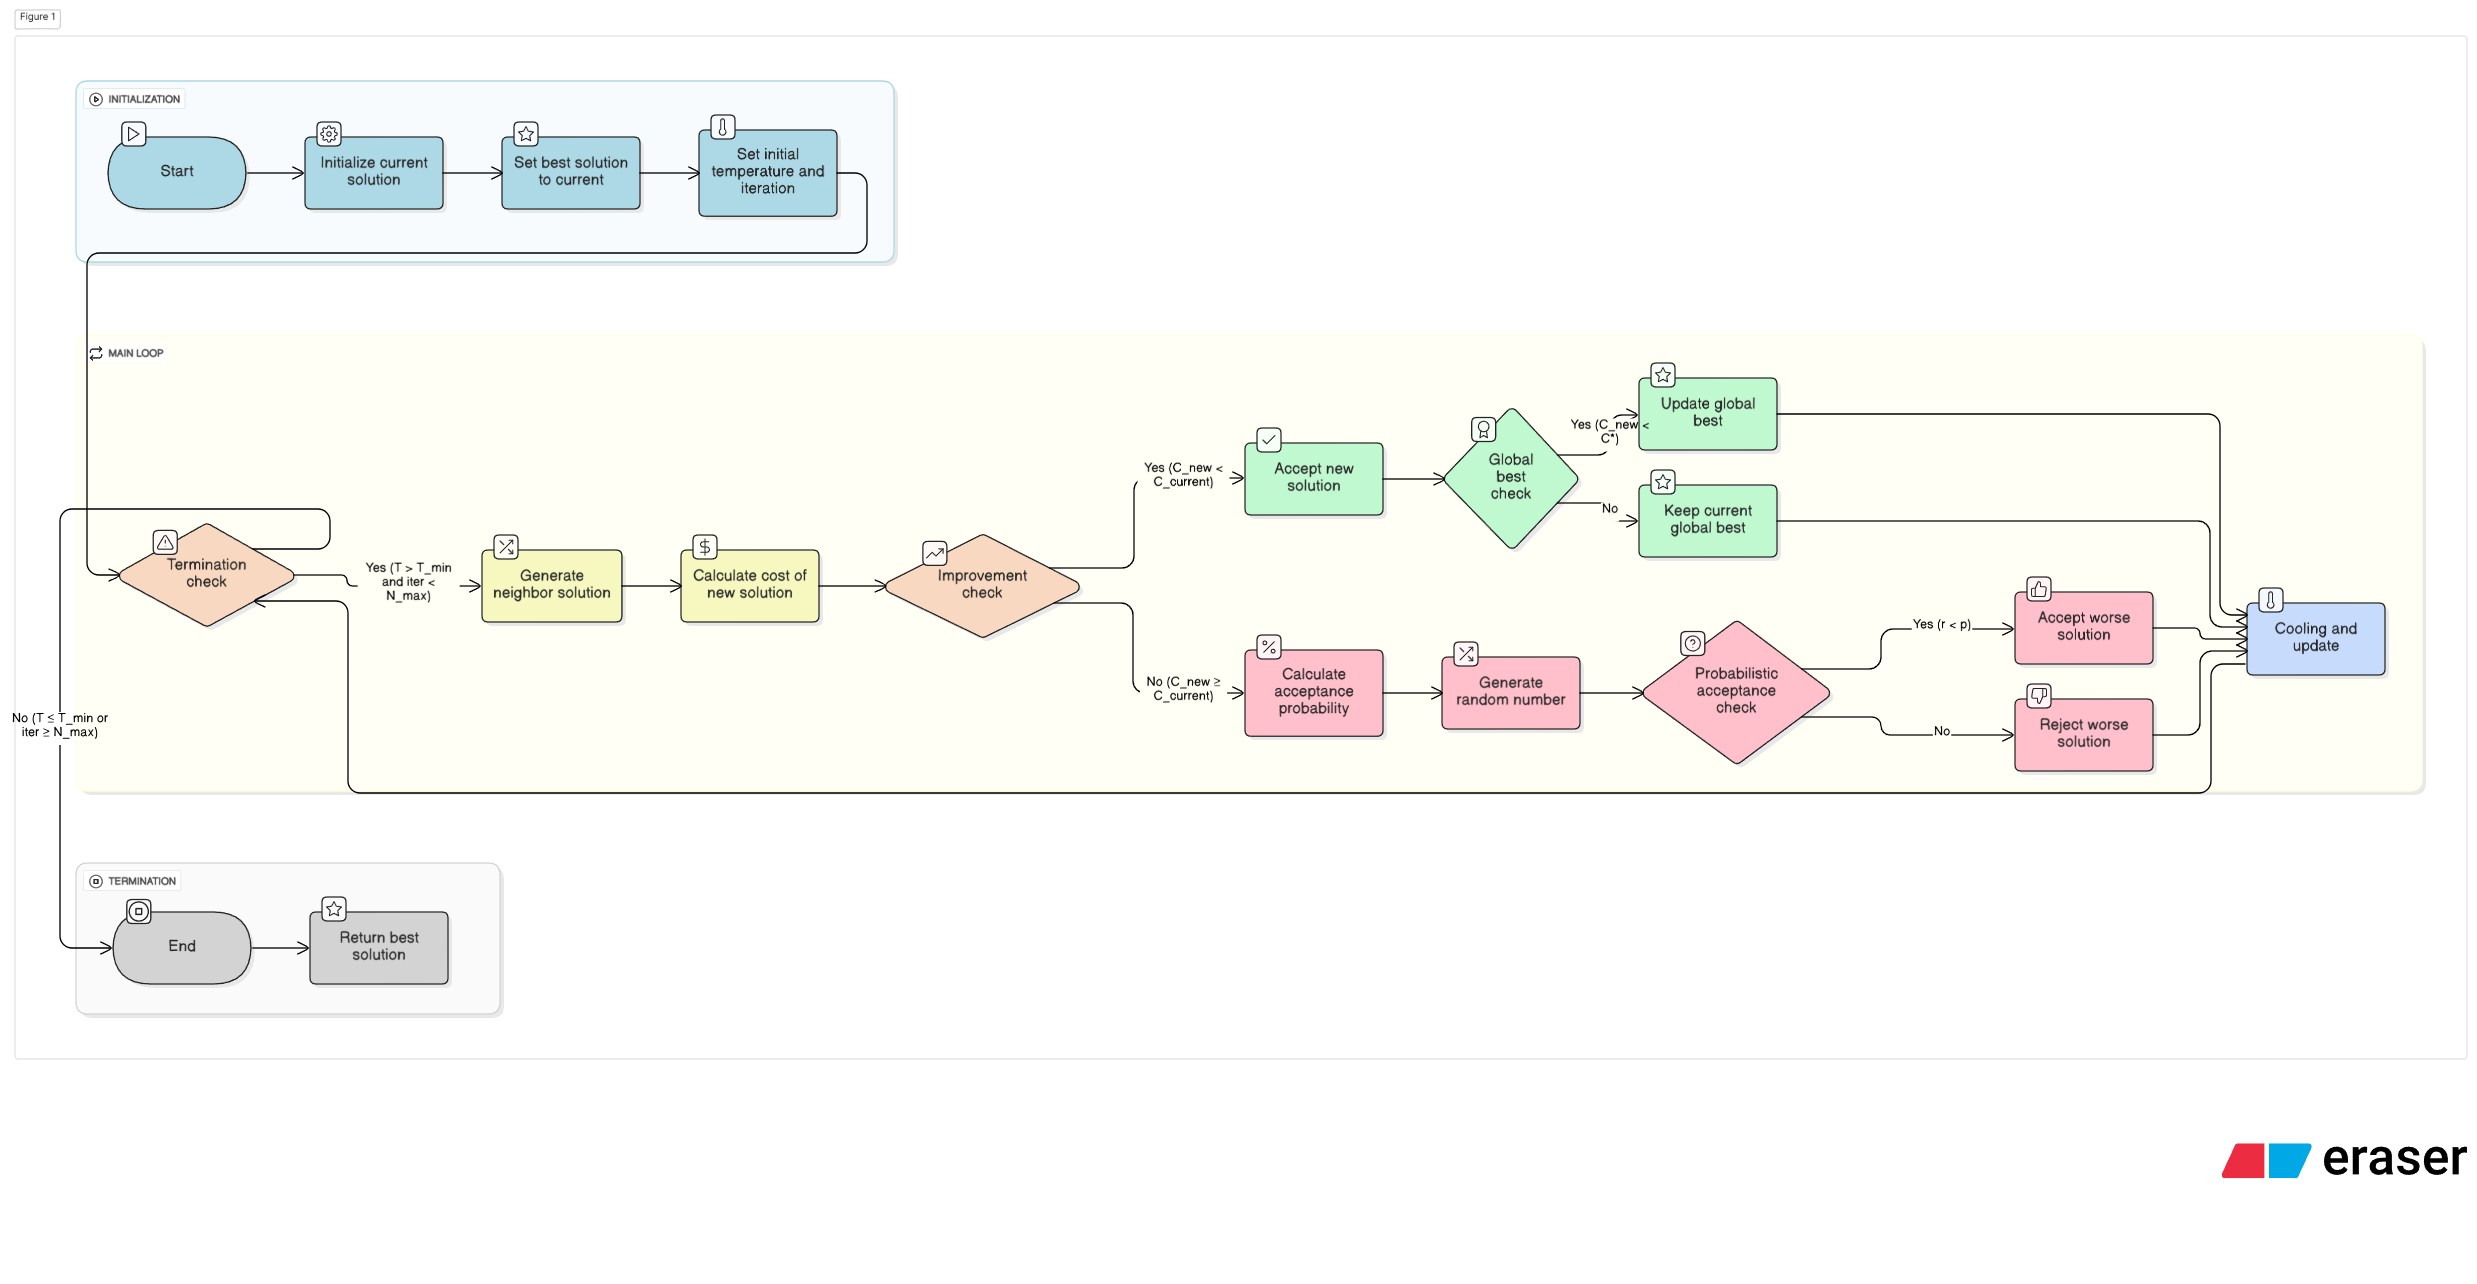
\includegraphics[width=0.8\textwidth]{Figures/flow_chart.png}
    \caption{Simulated Annealing algorithm flowchart for multi-robot path planning.}
    \label{fig:sa_flowchart}
\end{figure}

\subsection{Problem-Specific Considerations}

\begin{itemize}
    \item \textbf{Neighborhood Operator:} Implemented in \texttt{generate\_neighbor()}, which randomly alters up to 15 movements per robot and ensures feasibility before returning the modified path.

    \item \textbf{Feasibility Check:} Conducted by \texttt{is\_feasible(path\_array)}, verifying that paths respect motion constraints, avoid collisions, remain within map bounds, and comply with energy limits.

    \item \textbf{Cooling Schedule:} The temperature $T$ is reduced geometrically using $T_{new} = T_{current} \times 0.995$, gradually limiting the acceptance of worse solutions as the algorithm progresses.
\end{itemize}

\subsection{GenerateNeighbor Subroutine}

\begin{algorithm}[H]
\caption{Generate Feasible Neighbor Solution}
\begin{algorithmic}[1]
\Require Current movements $M_{current}$, maximum retries $R_{max}$
\Ensure Feasible neighbor movements $M_{neighbor}$

\For{$attempt \gets 1$ \textbf{to} $R_{max}$}
    \State $M_{new} \gets \text{Copy}(M_{current})$ \Comment{Deep copy}
    
    \For{each robot $r$}
        \For{$i \gets 1$ \textbf{to} 15} \Comment{Modify 15 random movements}
            \State $idx \gets \text{RandomInt}(0, K-1)$ \Comment{Random step index}
            \State $M_{new}[r][idx] \gets \text{RandomInt}(0, 4)$ \Comment{Random direction: 0=stay, 1-4=move}
        \EndFor
    \EndFor
    
    \State $P_{new} \gets \text{MovementsToPositions}(M_{new})$
    \If{$\text{IsFeasible}(P_{new})$} \Comment{Check for collisions}
        \State \Return $M_{new}$ \Comment{Valid neighbor found}
    \EndIf
\EndFor

\State \textbf{Warning:} No feasible neighbor found
\State \Return $M_{current}$ \Comment{Return original if all attempts fail}
\end{algorithmic}
\end{algorithm}

\subsection{Key Algorithm Components}

\subsubsection{Cost Function}
The cost function is designed as a \textbf{minimization problem}:
\begin{equation}
\text{Cost}(P) = -\alpha \cdot \text{Coverage}(P) + \beta \cdot \text{PathLength}(P)
\end{equation}

where:
\begin{itemize}
    \item $\text{Coverage}(P)$: Percentage of area covered by robots
    \item $\text{PathLength}(P)$: Total path length traveled
    \item $\alpha$: Weight for coverage (negative to maximize coverage)
    \item $\beta$: Weight for path smoothness
\end{itemize}

\textbf{Lower cost is better} - the algorithm minimizes this cost function.

\subsubsection{Acceptance Probability}
The Metropolis criterion for accepting worse solutions:
\begin{equation}
P(\text{accept}) = \begin{cases}
1 & \text{if } C_{new} < C_{current} \\
\exp\left(-\frac{C_{new} - C_{current}}{T}\right) & \text{otherwise}
\end{cases}
\end{equation}

As temperature $T$ decreases:
\begin{itemize}
    \item Early iterations: High $T$ allows exploration (accepts many worse solutions)
    \item Late iterations: Low $T$ focuses on exploitation (rarely accepts worse solutions)
\end{itemize}

\subsubsection{Cooling Schedule}
Geometric cooling is used:
\begin{equation}
T_{k+1} = \alpha \cdot T_k
\end{equation}

where $\alpha$ is the cooling rate (typically 0.995 in your implementation).

\subsubsection{Neighbor Generation Strategy}
For each robot, 15 random movement steps are modified:
\begin{itemize}
    \item Movement values: 0 (stay), 1 (up), 2 (down), 3 (left), 4 (right)
    \item Feasibility check: Ensures no robot collisions
    \item Maximum 100 retries to find valid neighbor
\end{itemize}

\subsubsection{Termination Criteria}
The algorithm stops when:
\begin{enumerate}
    \item Temperature drops below $T_{min}$, \textbf{OR}
    \item Maximum iterations $N_{max}$ is reached
\end{enumerate}

\section{Genetic Algorithm Implementation}

The implemented \textbf{Genetic Algorithm (GA)} algorithm optimizes the movement sequences of six robots over 125 time steps on a $20 \times 20$ grid. The algorithm begins from a feasible random population, and then does several generational updates by mutation and crossover methods searching the solution landscape until it reaches the optimal solution.Each candidate path is validated against energy, collision, and obstacle constraints.

Solutions are evaluated using the following cost function:
\[
\text{Cost} = \frac{\alpha}{\text{Coverage}} + \frac{\beta}{\text{Connectivity}} + \gamma \cdot P_{\text{disconnect}}
\]
where $\alpha=3000$, $\beta=500$, and $\gamma=4.0$ weight coverage, connectivity, and disconnection penalties respectively.  

The algorithm chooses a certain percentage of chromosomes (solutions) per population as elites, where they are propagated to the next iteration, since they have the best fitness value (lowest cost). It selects another percentage of individuals to mutate, and those are the worst fitness individuals. Then, parents are selected from the remaining solutions to perform crossover.

\subsection{Pseudocode}

\begin{algorithm}[H]
\caption{Genetic Algorithm for Multi-Robot Path Planning}
\begin{algorithmic}[1]
\State \textbf{Input:} Initial solution, Robot positions, Population size $m$, Generation size $i_{max}$
\State \textbf{Input:} Elite rate $p_e$, Mutation rate $p_m$, Objective function $f(\mathbf{x})$
\State \textbf{Initialize:} Generate initial population from initial solution
\State \textbf{Initialize:} Best solution $\mathbf{x}^*$, Best cost $f^* = \infty$

\While{$i \leq i_{max}$}
    \State \textbf{// Evaluate Fitness}
    \For{each individual in population}
        \State Compute fitness: $fitness = f(\mathbf{x})$
        \State Store fitness in fitness\_list
    \EndFor
    
    \State \textbf{// Update Best Solution}
    \State $current\_cost = \min(fitness\_list)$
    \State $current\_solution = population[argmin(fitness\_list)]$
    \If{$current\_cost < f^*$}
        \State $f^* = current\_cost$
        \State $\mathbf{x}^* = current\_solution$
    \EndIf
    
    \State \textbf{// Generate New Population}
    \State $new\_population = []$
    
    \State \textbf{// Elitism: Select top $p_e \times m$ survivors}
    \State Sort population by fitness
    \State $elites = $ top $p_e \times m$ individuals
    \State Add $elites$ to $new\_population$
    
    \State \textbf{// Mutation: Mutate worst $p_m \times m$ individuals}
    \State $worst\_individuals = $ bottom $p_m \times m$ individuals
    \For{each individual in worst\_individuals}
        \State Apply swap mutation per robot path
        \State Ensure mutated individual is feasible
        \State Add mutated individual to $new\_population$
    \EndFor
    
    \State \textbf{// Crossover: Generate offspring for remaining slots}
    \State $num\_crossover = m - |new\_population|$
    \State $offspring\_count = 0$
    \While{$offspring\_count < num\_crossover$}
        \State Select 2 parents using Stochastic Universal Sampling (SUS)
        \State Apply one-point crossover per robot path
        \State Generate $offspring_1, offspring_2$
        \State Filter feasible offspring
        \State Sort feasible offspring by fitness
        \If{feasible offspring exist}
            \State Add fittest offspring to $new\_population$
            \State $offspring\_count = offspring\_count + 1$
        \EndIf
    \EndWhile
    
    \State $population = new\_population$
    \State $i = i + 1$
\EndWhile

\State \textbf{Output:} Best solution $\mathbf{x}^*$, Best cost $f^*$
\end{algorithmic}
\end{algorithm}

\subsection{Problem-Specific Considerations}
\begin{itemize}
    \item \textbf{Crossover Operator:} Implemented using one-point crossover per robot path in \\ \texttt{one\_point\_crossover\_for\_robots\_paths()}, which selects a random crossover point for each robot's path independently and exchanges segments between two parent solutions to create offspring.
    \item \textbf{Mutation Operator:} Implemented using swap mutation per robot path in \\ \texttt{swap\_mutation\_per\_robot\_path()}, which randomly swaps two positions within each robot's path independently to introduce variation.
    \item \textbf{Parent Selection:} Implemented using Stochastic Universal Sampling (SUS) in \\ \texttt{select\_parents\_by\_sus()}, which uses evenly-spaced pointers to select parents proportionally to their fitness, providing better diversity than roulette wheel selection.
    \item \textbf{Feasibility Check:} Conducted by \texttt{is\_feasible(path\_array)} throughout the genetic operations, verifying that generated offspring and mutated individuals respect motion constraints, avoid collisions, remain within map bounds, and comply with energy limits. Infeasible solutions are rejected and regenerated.
    \item \textbf{Elite Preservation:} The top $p_e \times m$ individuals (fittest solutions) are directly carried over to the next generation to preserve high-quality solutions.
\end{itemize}

\section{Ant Colony Optimization Implementation}

The \textbf{Ant Colony Optimization (ACO)} module constructs paths for all robots by sampling movements for a population of ants while maintaining a global pheromone map. Each ant independently samples a path using either a pheromone-only strategy (\texttt{SACO}) or the Ant System variant (\texttt{AS}) that mixes pheromone strength with a heuristic map. After every iteration, pheromones evaporate globally and are reinforced along the best path of the iteration; local pheromone updates occur either per move (\texttt{AS}) or once per constructed path (\texttt{SACO}). Heuristic desirability is pre-computed so that unexplored cells receive higher weight than free space and obstacles.

\subsection{Pseudocode}

\begin{algorithm}[H]
\caption{Ant Colony Optimization for Multi-Robot Path Planning}
\begin{algorithmic}[1]
\State \textbf{Input:} Number of ants $m$, iterations $N_{max}$, $\alpha_{\tau}$ (pheromone weight), $\beta_{\eta}$ (heuristic weight), evaporation rate $\rho$, strategy $\in\{$SACO, AS$\}$
\State Initialize pheromone map $\tau$ to $1.0$ for all cells; build heuristic map $\eta$ (unexplored $>$ free $>$ obstacle)
\State \textbf{Initialize:} $best\_cost \gets \infty$, $best\_path \gets \varnothing$
\For{$iter = 1$ to $N_{max}$}
    \State Apply evaporation: $\tau \gets (1-\rho)\cdot \tau$
    \For{ant $k = 1$ to $m$}
        \For{each robot $r$}
            \State $p \gets$ initial position of robot $r$
            \For{$t = 1$ to $K$ steps}
                \State $F \gets$ feasible moves from $p$ (stay or 4-connected within bounds)
                \State Compute weight $w = \tau^{\alpha_{\tau}} \cdot \eta^{\beta_{\eta}}$ for each move (omit $\eta$ when SACO)
                \State Sample move via roulette-wheel on $w$
                \State Apply move, update $p$; if AS, apply local decay on $\tau$ at $p$
            \EndFor
        \EndFor
        \State Build full path $P_k$, compute cost $C_k$ with coverage/connectivity penalties
        \State Local deposit along $P_k$ (pheromone-only or heuristic-weighted)
    \EndFor
    \State Select iteration best $(P^*, C^*)$; reinforce $\tau$ along $P^*$ (AS) while evaporating
    \If{$C^* < best\_cost$} \State $best\_cost \gets C^*$, $best\_path \gets P^*$ \EndIf
    \State Record metrics / visualization
\EndFor
\State \textbf{Return} $best\_path$, $best\_cost$
\end{algorithmic}
\end{algorithm}

\subsection{Implementation Details}
\begin{itemize}
    \item \textbf{Move sampling:} \texttt{AntColonyStrategy.select\_move()} computes weights from $\tau^{\alpha_{\tau}}$ (SACO) or $\tau^{\alpha_{\tau}}\eta^{\beta_{\eta}}$ (AS). Moves are drawn with roulette-wheel sampling; if all weights vanish, a random feasible move is chosen.
    \item \textbf{Heuristic map:} \texttt{\_build\_heuristic\_map()} assigns 2.0 to unexplored, 1.2 to free space, and $10^{-6}$ to obstacles to discourage infeasible cells.
    \item \textbf{Evaporation and updates:} \texttt{before\_iteration()} applies uniform evaporation. \texttt{ASStrategy.local\_after\_move()} applies per-move decay toward the initial pheromone. Both strategies call \texttt{update\_local\_pheromone()} after constructing a full path, depositing $(1/(1+\text{cost}))$ on visited cells (scaled by heuristic for AS).
    \item \textbf{Global reinforcement:} \texttt{ASStrategy.after\_iteration()} reinforces the iteration-best path with factor $(1+\beta_{\eta})/(1+\text{cost})$ while re-applying evaporation; SACO relies solely on local deposits plus the global evaporation step.
    \item \textbf{Feasibility:} \texttt{\_get\_feasible\_moves()} restricts motion to in-bounds 4-connected moves; collision/energy/obstacle feasibility is enforced in the shared cost function.
    \item \textbf{Interfaces:} Inherits visualization/cost utilities from \texttt{BaseOptimizer}; maintains ant moves as an $(m \times R \times K)$ array and converts to positions with \texttt{movements\_to\_positions()} for scoring.
\end{itemize}
